\documentclass[12pt]{article}

\usepackage{amsmath, mathtools}
\usepackage{amsfonts}
\usepackage{amssymb}
\usepackage{graphicx}
\usepackage{colortbl}
\usepackage{xr}
\usepackage{hyperref}
\usepackage{longtable}
\usepackage{xfrac}
\usepackage{tabularx}
\usepackage{float}
\usepackage{siunitx}
\usepackage{booktabs}
\usepackage{caption}
\usepackage{pdflscape}
\usepackage{afterpage}
\usepackage{hyperref}
\usepackage{multirow}
\usepackage{array}
\usepackage{enumitem}

\usepackage[round]{natbib}

%\usepackage{refcheck}

\hypersetup{
    bookmarks=true,         % show bookmarks bar?
      colorlinks=true,       % false: boxed links; true: colored links
    linkcolor=red,          % color of internal links (change box color with linkbordercolor)
    citecolor=green,        % color of links to bibliography
    filecolor=magenta,      % color of file links
    urlcolor=cyan           % color of external links
}

%% Comments

\usepackage{color}

\newif\ifcomments\commentstrue %displays comments
%\newif\ifcomments\commentsfalse %so that comments do not display

\ifcomments
\newcommand{\authornote}[3]{\textcolor{#1}{[#3 ---#2]}}
\newcommand{\todo}[1]{\textcolor{red}{[TODO: #1]}}
\else
\newcommand{\authornote}[3]{}
\newcommand{\todo}[1]{}
\fi

\newcommand{\wss}[1]{\authornote{blue}{SS}{#1}} 
\newcommand{\plt}[1]{\authornote{magenta}{TPLT}{#1}} %For explanation of the template
\newcommand{\an}[1]{\authornote{cyan}{Author}{#1}}

%% Common Parts

\newcommand{\progname}{Sayyara Automotive Matcher} % PUT YOUR PROGRAM NAME HERE
\newcommand{\authname}{Team 27, Kappastone
\\ Tevis Doe, doet
\\ Caitlin Bridel, bridelc
\\ Gilbert Cherrie, cherrieg
\\ Rachel Johnson, johnsr12
\\ Harkeerat Kanwal, kanwalh
\\ Himanshu Aggarwal, aggarwah} % AUTHOR NAMES                  

\usepackage{hyperref}
    \hypersetup{colorlinks=true, linkcolor=blue, citecolor=blue, filecolor=blue,
                urlcolor=blue, unicode=false}
    \urlstyle{same}
                                


% For easy change of table widths
\newcommand{\colZwidth}{1.0\textwidth}
\newcommand{\colAwidth}{0.13\textwidth}
\newcommand{\colBwidth}{0.82\textwidth}
\newcommand{\colCwidth}{0.1\textwidth}
\newcommand{\colDwidth}{0.05\textwidth}
\newcommand{\colEwidth}{0.8\textwidth}
\newcommand{\colFwidth}{0.17\textwidth}
\newcommand{\colGwidth}{0.5\textwidth}
\newcommand{\colHwidth}{0.28\textwidth}

% Used so that cross-references have a meaningful prefix
\newcounter{defnum} %Definition Number
\newcommand{\dthedefnum}{GD\thedefnum}
\newcommand{\dref}[1]{GD\ref{#1}}
\newcounter{datadefnum} %Datadefinition Number
\newcommand{\ddthedatadefnum}{DD\thedatadefnum}
\newcommand{\ddref}[1]{DD\ref{#1}}
\newcounter{theorynum} %Theory Number
\newcommand{\tthetheorynum}{T\thetheorynum}
\newcommand{\tref}[1]{T\ref{#1}}
\newcounter{tablenum} %Table Number
\newcommand{\tbthetablenum}{T\thetablenum}
\newcommand{\tbref}[1]{TB\ref{#1}}
\newcounter{assumpnum} %Assumption Number
\newcommand{\atheassumpnum}{P\theassumpnum}
\newcommand{\aref}[1]{A\ref{#1}}
\newcounter{goalnum} %Goal Number
\newcommand{\gthegoalnum}{P\thegoalnum}
\newcommand{\gsref}[1]{GS\ref{#1}}
\newcounter{instnum} %Instance Number
\newcommand{\itheinstnum}{IM\theinstnum}
\newcommand{\iref}[1]{IM\ref{#1}}
\newcounter{reqnum} %Requirement Number
\newcommand{\rthereqnum}{P\thereqnum}
\newcommand{\rref}[1]{R\ref{#1}}
\newcounter{ucnum} %Use Case Number
\newcommand{\rtheucnum}{P\theucnum}
\newcommand{\ucref}[1]{R\ref{#1}}
\newcounter{nfrnum} %NFR Number
\newcommand{\rthenfrnum}{NFR\thenfrnum}
\newcommand{\nfrref}[1]{NFR\ref{#1}}
\newcounter{lcnum} %Likely change number
\newcommand{\lthelcnum}{LC\thelcnum}
\newcommand{\lcref}[1]{LC\ref{#1}}

\usepackage{fullpage}

\newcommand{\deftheory}[9][Not Applicable]
{
\newpage
\noindent \rule{\textwidth}{0.5mm}

\paragraph{RefName: } \textbf{#2} \phantomsection 
\label{#2}

\paragraph{Label:} #3

\noindent \rule{\textwidth}{0.5mm}

\paragraph{Equation:}

#4

\paragraph{Description:}

#5

\paragraph{Notes:}

#6

\paragraph{Source:}

#7

\paragraph{Ref.\ By:}

#8

\paragraph{Preconditions for \hyperref[#2]{#2}:}
\label{#2_precond}

#9

\paragraph{Derivation for \hyperref[#2]{#2}:}
\label{#2_deriv}

#1

\noindent \rule{\textwidth}{0.5mm}

}

\begin{document}

\title{Software Requirements Specification for \progname: subtitle describing software} 
\author{\authname}
\date{\today}
	
\maketitle

~\newpage

\pagenumbering{roman}

\tableofcontents

~\newpage

\section*{Revision History}

\begin{tabularx}{\textwidth}{p{3cm}p{2cm}X}
\toprule {\bf Date} & {\bf Version} & {\bf Notes}\\
\midrule
5 October 2022 & 1.0 & First iteration of SRS\\
Date 2 & 1.1 & Notes\\
\bottomrule
\end{tabularx}
\\\\
This SRS closely follows the Volere template provided by the course instructor, however it uses some parts of the initial template as well. However, it covers the same sections as both templates, so no big changes have actually occurred. Some of the subsections that were not relevant to the project were omitted from these templates.

~\newpage

\section{Reference Material}

This section records information for easy reference.

\subsection{Table of Units}

N/A

\subsection{Table of Symbols}

N/A

\subsection{Abbreviations and Acronyms}

\renewcommand{\arraystretch}{1.2}
\begin{tabular}{l l} 
  \toprule		
  \textbf{symbol} & \textbf{description}\\
  \midrule 
  A & Assumption\\
  FR & Functional Requirement\\
  NFR & Non-Functional Requirement\\
  SRS & Software Requirements Specification\\
  PWA & Progressive Web App\\
  MVP & Minimal Viable Product\\
  AWS & Amazon Web Services\\
  URL & Uniform Resource Locator\\
  \bottomrule
\end{tabular}\\
\subsection{Mathematical Notation}

N/A

\newpage

\pagenumbering{arabic}

\section{Introduction}

This section provides an overview of the rest of the document. It describes the purpose of this document, outlines the expected knowledge of the reader and provides a roadmap of the SRS.

\subsection{Purpose of Document}

  The purpose of this document is to present a detailed description of \progname{} and outline the expectations of the program for functionality and performance. The document will describe the purpose of the system and its features and constraints. This SRS will also indicate conditions under which the system will be developed. This document is intended to be read by stakeholders and developers to achieve a better understanding of the system.

\subsection{Characteristics of Intended Reader} \label{sec_IntendedReader}

  The intended audience for this document are developers and other stakeholders such as project managers, quality assurance and product experts. It is assumed that these readers have a basic understanding of Progressive Web App (PWA) development and server hosting. It is also assumed that the reader understands the process for car maintenance, including quotes, work orders and billing.

\subsection{Organization of Document}

  The document is divided into sections that each give an in-depth look into an aspect of the system. To begin, the \hyperref[sec:GSD]{General System Description} section describes the system and identifies how it will interact with its environment and users. This section will also summarize the attributes of the expected users. The following section, \hyperref[sec:SSD]{Specific System Description}, will describe the purpose of the system through the problem statement and explain necessary terminology for complete understanding of the problem and requirements. The \hyperref[sec:FuncReq]{Functional Requirements} section will outline the needs of the client and expectations of the software, in terms of functionality. This section will also describe the scope of work, formal requirements and the plan for how the team intends to implement the functional requirements. Following that, the \hyperref[sec:NFuncReq]{Nonfunctional Requirements} section will explain all quality features the team plans to implement in this project. The current environment for this system will be discussed in the \hyperref[sec:PI]{Project Issues} section, to present all factors that will contribute to the success or potential failure of \progname{}. Finally, the \hyperref[sec:refAppendix]{Reflection Appendix} details the skills and knowledge each team member requires in order to complete this project and the proposed action plan accepted by each member. 

\section{General System Description} \label{sec:GSD}

This section provides general information about the system.  It identifies the
interfaces between the system and its environment, describes the user
characteristics and lists the system constraints.

\subsection{System Context} \label{sec:SystemContext}

The system context for this PWA is shown in Figure 1. This figure shows the relationship between the user inputs and the different parts of the software that the users interact with. The figure starts at the User box which shows the first stage of user input which is the user logging in as a customer, shop owner or shop employee. From this stage they are guided to the respective front end view of the PWA relevant to their access level and from these front end PWA views they have various interactions and user inputs that will interact with the database and have various outputs as shown by the arrows in the figure.

\begin{figure}[h!]
\begin{center}
 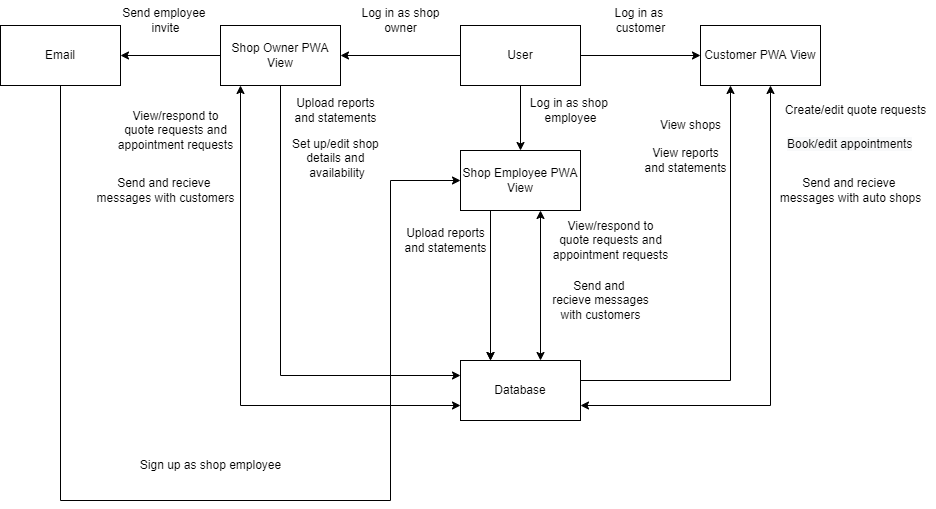
\includegraphics[width=1\textwidth]{SystemContext}
\caption{System context displaying user interactions with PWA views and database. }
\label{Fig_SystemContext} 
\end{center}
\end{figure}

\subsection{User Characteristics} \label{SecUserCharacteristics}

The end users of the system can be of two types, a typical consumer and a typical shop owner or employee. The general consumer will not be expected to have any knowledge about auto motives, and as such it will not be required to use the software. In general, the typical consumer is expected to know how to use a mobile app or web page (which will be the output of this project, see \hyperref[constraints]{System Constraints}) without any instruction. Finally, general consumers are assumed to have no physical disabilities that may prevent them from using the system. 

Shop owners/employees are expected to have all the same general knowledge as a typical consumer but with knowledge relating to the automotive industry in addition. In particular, this type of user will have knowledge about the terminology and processes used in the auto motive industry, and as such, they will not be explained to any potential users. Shop owners or employees are expected have the knowledge to be able to assist consumers in their understanding of auto motives to allow them to more effectively use the application.

\subsection{System Constraints}
\label{constraints}

This system has no constraints, barring one. The output of the project, as mandated by the supervisor of the project, will be a PWA (progressive web app). This means that the output of the project will take the form both of a web page that can be run in a browser, but also an application that will run on mobile devices. 

\section{Specific System Description} \label{sec:SSD}

This section presents the problem description, which gives a high-level view of the problem to be solved. In addition, it contains a section detailing any terminology used in the document that may be unclear for readers.

\subsection{Problem Description} \label{Sec_pd}

\progname{} is intended to solve a typical issue that a consumer may run in to when attempting to service their vehicle: finding a reliable mechanic, and creating appointments with them. Consumers may have to phone many mechanics to find a mechanic that charges a reasonable price for services, and may not necessarily even be able to find a time slot that works for both the mechanic and them. \progname intends to solve these issues with coordination for both consumers and mechanics, making servicing vehicles easier for the both of them.

\subsubsection{Terminology and  Definitions}

This subsection provides a list of terms that are used in the subsequent
sections and their meaning, with the purpose of reducing ambiguity and making it
easier to correctly understand the requirements:

\begin{itemize}

\item \label{term_cannedJob} Canned job: a job provided by a shop where the pricing and timing is already listed, so there is no need for a customer to request a quote or for the shop to send a quote to the customer.

\end{itemize}

\subsection{Solution Characteristics Specification}

This section covers the assumptions that may affect the requirements if changed in the future.

\subsubsection{Assumptions}

Many assumptions about the users of the system are detailed under \hyperref[SecUserCharacteristics]{User Characteristics}, but the following assumptions are also made:

\begin{itemize}
    \item The mobile hardware that a user has will support PWAs.
    \item When using the application, the user will have a valid internet connection.
    \item The servers that eventually host the system will be able to support the users of the system.
\end{itemize}

\noindent If there is a change in these assumptions, the functional requirements defined in the following section may be subject to change.

\section{Functional Requirements} \label{sec:FuncReq}

This section provides the functional requirements, the business tasks that the
software is expected to complete, and the nonfunctional requirements, the
qualities that the software is expected to exhibit.

\subsection{The Scope of the Work and the Product}

\subsubsection{The Context of the Work}

The system context is covered in Section \ref{sec:SystemContext}

\subsubsection{Work Partitioning}

The work partitioning is outlined in Table \ref{tab:WorkPartitioning}.

\begin{center}
\begin{longtable}{|p{4cm}|p{5cm}|p{6cm}|}
\caption{Work Partitioning}
\label{tab:WorkPartitioning} \\
\hline
 \textbf{Event} & \textbf{Input and Output} & \textbf{Summary} \\
\hline
Create account & User info (IN) & User creates account \\
\hline
User logs in & Username (IN) & User logs into the system \\
 & Password (IN) & \\
\hline
Reset password & New password (IN) & User resets password \\
\hline
Enroll shop & Shop name (IN) & Shop owner enrolls store \\
 & Shop address (IN) & \\
 & Owner info (IN) & \\
\hline
Owner invites employee & Employee (IN) & Owner invites employee to create account \\
& Employee invite (OUT) & \\
\hline
View all users & All users (OUT) & System admin views all mechanics and users \\
\hline
Send quote request & Quote request (IN) & Customer sends quote request to shop \\
 & Quote from shop (OUT) & \\
\hline
Book appointment & Appointment request (IN) & Customer books appointment with shop \\
 & Appointment acceptance/rejection (OUT) & \\
\hline
Create work order & Customer and quote info (IN) & Shop creates work order \\
 & Work order (OUT) & \\
\hline
Assign work order & Employee (IN) & Shop owner assigns work order to employee \\
 & Work order (IN) & \\
\hline
Cancel appointment & Appointment (IN) & Shop owner cancels appointment \\
\hline
Set shop availability & Shop available hours/days (IN) & Shop sets shop availability \\
 & Shop schedule (OUT) & \\
\hline
\end{longtable}
\end{center}

\subsubsection{Individual Product Use Cases}

\noindent \begin{itemize}

\item[UC\refstepcounter{ucnum}\theucnum \label{UC_EnrollShop}. ]
Name: Enroll Shop\\
Trigger: Shop owner attempts to enroll shop\\
Precondition: None\\
Main Success Scenario:
\begin{enumerate}
    \item Shop owner enters required information
\end{enumerate}
Success Postcondition: Shop owner successfully enrolls shop\\
Functional Requirement(s): FR\ref{R_EnrollShop}

\item[UC\refstepcounter{ucnum}\theucnum \label{UC_CreateOwnerAccount}. ]
Name: Create Owner Account\\
Trigger: Shop owner attempts to create account\\
Precondition: Shop owner enrolls shop\\
Main Success Scenario:
\begin{enumerate}
    \item Shop owner enters required information
\end{enumerate}
Success Postcondition: Shop owner successfully creates account
Functional Requirement(s): FR\ref{R_CreateOwnerAccount}

\item[UC\refstepcounter{ucnum}\theucnum \label{UC_CreateEmployeeAccount}. ]
Name: Create Employee Account\\
Trigger: Shop employee attempts to create account\\
Precondition: Shop owner invites employee to create account\\
Main Success Scenario:
\begin{enumerate}
    \item Shop employee accepts invitation from shop owner
    \item Shop employee enters required information
\end{enumerate}
Success Postcondition: Shop employee successfully creates account\\
Functional Requirement(s): FR\ref{R_InviteEmployee}, FR\ref{R_CreateEmployeeAccount}, FR\ref{R_EditEmployee}

\item[UC\refstepcounter{ucnum}\theucnum \label{UC_Login}. ]
Name: Login\\
Trigger: User attempts to login\\
Precondition: User creates account\\
Main Success Scenario:
\begin{enumerate}
    \item User enters username and password
    \item System authenticates username and password
\end{enumerate}
Undesired Event Handling:
\begin{enumerate}
    \item System cannot authenticate username or password
    \item User repeats Step 2 until successful authentication
\end{enumerate}
Success Postcondition: User successfully logs into account\\
Functional Requirement(s): FR\ref{R_Login}

\item[UC\refstepcounter{ucnum}\theucnum \label{UC_ViewAllUsers}. ]
Name: View All Users\\
Trigger: System admin attempts to view all mechanics and users\\
Precondition: System admin authenticates admin status\\
Success Postcondition: System admin successfully views all mechanics and users\\
Functional Requirements(s): FR\ref{R_SeeAllUsers}

\item[UC\refstepcounter{ucnum}\theucnum \label{UC_EditAccount}. ]
Name: Edit Account\\
Trigger: User attempts to edit account\\
Precondition: User logs into account\\
Main Success Scenario:
\begin{enumerate}
    \item User enters changes to account
    \item User saves changes
\end{enumerate}
Success Postcondition: User changes to account become visible\\
Functional Requirement(s): FR\ref{R_EditAccount}

\item[UC\refstepcounter{ucnum}\theucnum \label{UC_DeleteAccount}. ]
Name: Delete Account\\
Trigger: User attempts to delete account\\
Precondition: User is not a shop owner\\
Success Postcondition: User account is no longer visible\\
Functional Requirement(s): FR\ref{R_DeleteAccount}

\item[UC\refstepcounter{ucnum}\theucnum \label{UC_ResetPassword}. ]
Name: Reset Password\\
Trigger: User attempts to reset password\\
Precondition: User creates account\\
Main Success Scenario:
\begin{enumerate}
    \item User enters contact information
    \item System authenticates that user info exists in records
    \item System allows user to reset password
\end{enumerate}
Undesired Event Handling:
\begin{enumerate}
    \item System unable to authenticate user
    \item User repeats Step 1 until authentication succeeds
\end{enumerate}
Success Postcondition: User successfully resets password\\
Functional Requirement(s): FR\ref{R_RestPassword}

\item[UC\refstepcounter{ucnum}\theucnum \label{UC_CustomerBooksAppointment}. ]
Name: Customer Books Appointment\\
Trigger: Customer books appointment with shop\\
Precondition: None\\
Main Success Scenario:
\begin{enumerate}
    \item Customer searches for and selects shop
    \item Customer sends quote request to shop
    \item Shop owner or employee creates quote
    \item Shop owner or employee sends quote to customer
    \item Customer accepts quote
    \item Shop owner or employee accepts appointment
    \item System automatically creates work order
\end{enumerate}
Alternate Scenario:
\begin{enumerate}
    \item Customer searches for and selects shop
    \item Customer books a canned job (see \ref{term_cannedJob})
    \item Shop owner or employee accepts appointment
    \item System automatically creates work order
\end{enumerate}
Undesired Event Handling:
\begin{enumerate}
    \item Customer rejects quote or shop rejects appointment
    \item No appointment created
\end{enumerate}
Success Postcondition: Customer successfully books appointment\\
Functional Requirement(s): FR\ref{R_CreateQuote}, FR\ref{R_SendQuote}, FR\ref{R_EmployeeAppointment}, FR\ref{R_ViewShop}, FR\ref{R_AutoCreateWorkOrder}, FR\ref{R_BookAppointment}, FR\ref{R_SubmitQuoteRequests}, FR\ref{R_SearchShop}

\item[UC\refstepcounter{ucnum}\theucnum \label{UC_CancelAppointment}. ]
Name: Shop Cancels Appointment\\
Trigger: Shop owner attempts to cancel appointment\\
Precondition: Customer or shop books appointment\\
Main Success Scenario:
\begin{enumerate}
    \item Shop owner searches for upcoming work order, quote, or appointment
    \item Shop owner views appointment
    \item Shop owner cancels appointment
    \item System automatically deletes work order
\end{enumerate}
Success Postcondition: Shop successfully cancels appointment\\
Functional Requirement(s): FR\ref{R_OwnerAppointment}, FR\ref{R_ViewQuotes}, FR\ref{R_ViewWorkOrder}, FR\ref{R_AutoDeleteWorkOrder}

\item[UC\refstepcounter{ucnum}\theucnum \label{UC_AssignWorkOrder}. ]
Name: Assign Work Order\\
Trigger: Shop owner attempts to assign work order to employee\\
Precondition: Work order has been created\\
Main Success Scenario:
\begin{enumerate}
    \item Shop owner searches for and selects employee
\end{enumerate}
Success Postcondition: Shop owner successfully assigns work order to employee\\
Functional Requirement(s): FR\ref{R_ViewEmployee}, FR\ref{R_AssignWorkOrder}

\item[UC\refstepcounter{ucnum}\theucnum \label{UC_SendWorkOrder}. ]
Name: Send Work Order\\
Trigger: Shop attempts to send work order to customer\\
Precondition: Shop owner or employee creates work order\\
Success Postcondition: Customer successfully receives work order\\
Functional Requirement(s): FR\ref{R_CreateWorkOrder}, FR\ref{R_SendWorkOrder}

\item[UC\refstepcounter{ucnum}\theucnum \label{UC_EditShopProfile}. ]
Name: Edit Shop Profile\\
Trigger: Shop owner attempts to edit shop profile\\
Precondition: Shop owner enrolls shop and creates account\\
Success Postcondition: Changes visible on shop profile\\
Functional Requirement(s): FR\ref{R_EditShopProfile}

\item[UC\refstepcounter{ucnum}\theucnum \label{UC_SetShopAvailability}. ]
Name: Set Shop Availability\\
Trigger: Shop owner or employee attempts to set shop availability\\
Precondition: Shop owner or employee creates account\\
Success Postcondition: Customers can view shop availability\\
Functional Requirement(s): FR\ref{R_SetShopAvailability}

\end{itemize}

\subsection{Functional Requirements}

\noindent \begin{itemize}

\item[FR\refstepcounter{reqnum}\thereqnum \label{R_EnrollShop}.] The system will allow shop owners to enroll their shops.\\
Use Case: UC\ref{UC_EnrollShop}

\item[FR\refstepcounter{reqnum}\thereqnum \label{R_CreateOwnerAccount}.] The system will allow shop owners to create individual accounts.\\
Use Case: UC\ref{UC_CreateOwnerAccount}

\item[FR\refstepcounter{reqnum}\thereqnum \label{R_InviteEmployee}.] The system will allow shop owners to invite employees to create individual accounts.\\
Use Case: UC\ref{UC_CreateEmployeeAccount}

\item[FR\refstepcounter{reqnum}\thereqnum \label{R_CreateEmployeeAccount}.] The system will allow shop employees to create individual accounts via employer invitation.\\
Use Case: UC\ref{UC_CreateEmployeeAccount}

\item[FR\refstepcounter{reqnum}\thereqnum \label{R_SeeAllUsers}.] The system will allow system admin to see all mechanics and users.\\
Use Case: UC\ref{UC_ViewAllUsers}

\item[FR\refstepcounter{reqnum}\thereqnum \label{R_EditAccount}.] The system will allow any user to edit their own account.\\
Use Case: UC\ref{UC_EditAccount}

\item[FR\refstepcounter{reqnum}\thereqnum \label{R_DeleteAccount}.] The system will allow shop employees to delete their own account.\\
Use Case: UC\ref{UC_DeleteAccount}

\item[FR\refstepcounter{reqnum}\thereqnum \label{R_Login}.] The system will allow shop owners and employees to login by entering a username and password.\\
Use Case: UC\ref{UC_Login}

\item[FR\refstepcounter{reqnum}\thereqnum \label{R_RestPassword}.] The system will allow shop owners and employees to reset their password.\\
Use Case: UC\ref{UC_ResetPassword}

\item[FR\refstepcounter{reqnum}\thereqnum \label{R_CreateQuote}.] The system will allow shop owners to create quotes.\\
Use Case: UC\ref{UC_CustomerBooksAppointment}

\item[FR\refstepcounter{reqnum}\thereqnum \label{R_SendQuote}.] The system will allow shop owners and employees to send quotes to customers.\\
Use Case: UC\ref{UC_CustomerBooksAppointment}

\item[FR\refstepcounter{reqnum}\thereqnum \label{R_OwnerAppointment}.] The system will allow shop owners to accept, reject, and assign appointments.\\
Use Case: UC\ref{UC_CancelAppointment}

\item[FR\refstepcounter{reqnum}\thereqnum \label{R_EditEmployee}.] The system will allow shop owners to add, remove, and view all employees.\\
Use Case: UC\ref{UC_CreateEmployeeAccount}

\item[FR\refstepcounter{reqnum}\thereqnum \label{R_ViewEmployee}.] The system will allow shop owners and employees to view, search for, and filter employees.\\
Use Case: UC\ref{UC_AssignWorkOrder}

\item[FR\refstepcounter{reqnum}\thereqnum \label{R_CreateWorkOrder}.] The system will allow shop owners and employees to create work orders.\\
Use Case: UC\ref{UC_SendWorkOrder}

\item[FR\refstepcounter{reqnum}\thereqnum \label{R_SendWorkOrder}.] The system will allow shop owners to send work orders to customers.\\
Use Case: UC\ref{UC_SendWorkOrder}

\item[FR\refstepcounter{reqnum}\thereqnum \label{R_EditShopProfile}.] The system will allow shop owners to edit their shop profile.\\
Use Case: UC\ref{UC_EditShopProfile}

\item[FR\refstepcounter{reqnum}\thereqnum \label{R_EmployeeAppointment}.] The system will allow shop employees to accept and view appointments.\\
Use Case: UC\ref{UC_CustomerBooksAppointment}

\item[FR\refstepcounter{reqnum}\thereqnum \label{R_SetShopAvailability}.] The system will allow shop employees to set shop availability.\\
Use Case: UC\ref{UC_SetShopAvailability}

\item[FR\refstepcounter{reqnum}\thereqnum \label{R_ViewShop}.] The system will allow any user to view shop profiles.\\
Use Case: UC\ref{UC_CustomerBooksAppointment}

\item[FR\refstepcounter{reqnum}\thereqnum \label{R_ReworkRequest}.] The system will allow customers to submit rework requests.

\item[FR\refstepcounter{reqnum}\thereqnum \label{R_ViewQuotes}.] The system will allow shop owners and employees to view, search for, and filter quotes.\\
Use Case: UC\ref{UC_CancelAppointment}

\item[FR\refstepcounter{reqnum}\thereqnum \label{R_ViewWorkOrder}.] The system will allow shop owners and employees to view, search for, and filter past and upcoming work orders.\\
Use Case: UC\ref{UC_CancelAppointment}

\item[FR\refstepcounter{reqnum}\thereqnum \label{R_CustomerCommunication}.] The system will allow shop owners and employees to call and chat with customers.

\item[FR\refstepcounter{reqnum}\thereqnum \label{R_AutoDeleteWorkOrder}.] The system will automatically delete a work order if the appointment is cancelled.\\
Use Case: UC\ref{UC_CancelAppointment}

\item[FR\refstepcounter{reqnum}\thereqnum \label{R_AutoCreateWorkOrder}.] The system will automatically create a work order if an appointment is created.\\
Use Case: UC\ref{UC_CustomerBooksAppointment}

\item[FR\refstepcounter{reqnum}\thereqnum \label{R_AssignWorkOrder}.] The system will allow shop owners and employees to assign work orders to employees.\\
Use Case: UC\ref{UC_AssignWorkOrder}

\item[FR\refstepcounter{reqnum}\thereqnum \label{R_BookAppointment}.] The system will allow customers to book appointments.\\
Use Case: UC\ref{UC_CustomerBooksAppointment}

\item[FR\refstepcounter{reqnum}\thereqnum \label{R_SubmitQuoteRequests}.] The system will allow customers to submit quote requests.\\
Use Case: UC\ref{UC_CustomerBooksAppointment}

\item[FR\refstepcounter{reqnum}\thereqnum \label{R_SearchShop}.] The system will allow customers to search for and filter shops.\\
Use Case: UC\ref{UC_CustomerBooksAppointment}

Note: These functional requirements were derived from a Confluence board \hyperref[1]{[1]} with all user features created by our supervisor.

\end{itemize}

\subsection{Formalized Requirements}

The following Parnas table, \hyperref[tab:formal]{Table 2}, will formalize the utilization of the system between customers and shop owners/employees, one of the most important parts of the system. It will use the following variables to represent interactions, with abbreviations as neccesary:

\begin{itemize}
    \item Stimulus:
    \begin{itemize}
        \item In\_Chat: The customer or shop opens a chat with each other.
        \item In\_CustomerR: The customer makes an appointment with a shop.
        \item In\_ShopR: The shop owner/employee accepts a customer request.
        \item In\_Complete: The appointment with a customer is marked as complete.
    \end{itemize}
    \item State:
    \begin{itemize}
        \item Init (I): Initial state, can be considered to be a landing page.
        \item ChatWin (CW): The customer can chat with the shop and vice versa.
        \item AppShop (AS): The shop can see an appointment request from the customer.
        \item AppAcc (AA): The customer can see their request has been accepted by the shop.
    \end{itemize}
\end{itemize}
\newpage
\begin{longtable}{| p{3cm} | p{1cm} | p{1cm}| p{1cm} | p{1cm}| p{1cm}| p{1cm}|}
\caption{Formalized subsection of the requirements space.}
\label{tab:formal}
\\ \hline
\textbf{} & \textbf{I} & \textbf{CW} &\textbf{AS} & \textbf{AA} & \textbf{CW \& AS}  & \textbf{CW \& AA} \\
\hline
\endfirsthead

\textbf{In\_Chat} & CW & - & CW \& AS  & CW \& AA & - & - \\
\hline
\textbf{In\_CustomerR} & AS & CW \& AS & -  & - & - & -  \\
\hline
\textbf{In\_ShopR} & - & - & AA & - & CW \& AA & - \\
\hline
\textbf{In\_Complete} & - & - & - & I & - & I \\
\hline
\end{longtable}

\subsection{Phase in Plan}

In this section, the functional requirements have been divided into batches of work based on the applications user stories. The division of batches and proposed dates are detailed in Table \hyperref[tab:phaseInPlan]{3}.

\begin{table}[ht!]
  \caption{Schedule of batches of work} \\
  \label{tab:phaseInPlan}
  \centering
  \begin{tabular}{l|p{0.23\textwidth}|p{0.4\textwidth}|p{0.18\textwidth}}
  \toprule
  \textbf{Batch} & \textbf{Description} & \textbf{Functional Requirements} & \textbf{Dates}\\
  \midrule
  1 & Shop Owner Account Creation and Shop Enrolment & FR\ref{R_EnrollShop}, FR\ref{R_CreateOwnerAccount}, FR\ref{R_Login}, FR\ref{R_RestPassword} & Oct. 24, 2022\\
  \hline
  2 & Basic Customer Services & FR\ref{R_CreateQuote}, FR\ref{R_SendQuote}, FR\ref{R_OwnerAppointment}, FR\ref{R_CreateWorkOrder}, FR\ref{R_SendWorkOrder}, FR\ref{R_EmployeeAppointment}, FR\ref{R_SetShopAvailability}, FR\ref{R_ViewShop}, FR\ref{R_ViewQuotes}, FR\ref{R_ViewWorkOrder}, FR\ref{R_CustomerCommunication}, FR\ref{R_AutoDeleteWorkOrder}, FR\ref{R_AutoCreateWorkOrder}, FR\ref{R_BookAppointment}, FR\ref{R_SubmitQuoteRequests}, FR\ref{R_SearchShop} & Nov. 21, 2022\\
  \hline
  3 & Employee Account Creation & FR\ref{R_InviteEmployee}, FR\ref{R_CreateEmployeeAccount} & Jan. 5, 2023 \\
  \hline
  4 & Shop Owner Capabilities & FR\ref{R_EditEmployee}, FR\ref{R_ViewEmployee}, FR\ref{R_AssignWorkOrder} & Feb. 7, 2023\\
  \hline
  5 & Finishing Touches & FR\ref{R_SeeAllUsers}, FR\ref{R_EditAccount}, FR\ref{R_DeleteAccount}, FR\ref{R_EditShopProfile}, FR\ref{R_ReworkRequest} & Mar. 20, 2023\\
  \bottomrule
  \end{tabular}
  
\end{table}

\section{Nonfunctional Requirements} 
\label{sec:NFuncReq}

\subsection{Look and Feel Requirements}
\subsubsection{Appearance Requirements}
\begin{enumerate}[label = NFR-\arabic*, left=\parindent, series=nfr]
    \item The product shall be visually appealing.
    \newline \textbf{Rationale}: To attract new shop owners and customers to sign up, it is important that the product appears visually appealing. 
    \newline \textbf{Fit Criterion}: Without any external prompt, 90\% of a sample group of representative users shall start using the product within a few minutes of their encounter.
    
    \item The product shall have a consistent appearance on all of the devices.
    \newline \textbf{Rationale}: It is important for the product to have a consistent appearance so that users can use their experience with the product on other devices. 
    \newline \textbf{Fit Criterion}: 95\% of a sample group of users shall agree that the product looks identical in appearance on different devices.

    \item The product shall allow the users to customize the appearance of the product.
    \newline \textbf{Rationale}: Since everyone has a difference taste, it is important for the product to offer customization options so that users can have a more personalized experience. 
    \newline \textbf{Fit Criterion}: The supervisor shall certify that the product is customizable.
\end{enumerate}

\subsubsection{Style Requirements}
\begin{enumerate}[nfr]
    \item The product shall feel professional and trustworthy.
    \newline \textbf{Rationale}: It is essential that the product appear professional and trustworthy in order to build up the trust of the users.
    \newline \textbf{Fit Criterion}: 85\% of a representative sample of users shall agree that the product feels professional and trustworthy, 
    \item The font and theme used shall be consistent throughout the app.
    \newline \textbf{Rationale}: It is important that the components adhere to the same fonts and styles to ensure that they complement one another.
    \newline \textbf{Fit Criterion}: 90\% of a representative sample of users shall not be able to discern any variations in font and theme of any of the elements of the product.
\end{enumerate}

\subsection{Usability and Humanity Requirements}
\subsubsection{Ease of Use Requirements}
\begin{enumerate}[nfr]
    \item The product shall be easy to use by anyone above the age of 16.
    \newline \textbf{Rationale}: Since the minimum driving age in most provinces is 16, the product shall be user friendly for everyone above this age.
    \newline \textbf{Fit Criterion}: 80\% of the representative users who are 16 or older shall be able to do the assigned tasks in the allotted time.
    \item The product shall be usable by people with a basic comprehension of the English language, without any prior training. 
    \newline \textbf{Rationale}: To target a diverse group of users from various educational backgrounds, the product must not require prior training or knowledge to operate.
    \newline \textbf{Fit Criterion}: Without any training, 90\% of a sample English-speaking group shall be able to navigate through the different services offered by the app. 
\end{enumerate}

\subsubsection{Personalization and Internationalization Requirements}
\begin{enumerate}[nfr]
    \item The product shall automatically save user preferences.
    \newline \textbf{Rationale}: Users should be able to exit the web app and return later or on a different device with the same settings applied. This saves them time from making modifications everytime they launch the web app.
    \newline \textbf{Fit Criterion}: The settings applied by a user shall automatically apply on other devices at least 90\% of the times. 
\end{enumerate}

\subsubsection{Learning Requirements}
\begin{enumerate}[nfr]
    \item The product shall require no external training to learn.
    \newline \textbf{Rationale}: Users should not have to spend time learning how to use the different services offered by the product.
    \newline \textbf{Fit Criterion}: 95\% of a sample group shall be able to use the different services offered by the product without any prior experience or training with the product.
\end{enumerate}

\subsubsection{Understandability and Politeness Requirements}
\begin{enumerate}[nfr]
    \item The product shall use icons and symbols that are widely recognized.
    \newline \textbf{Rationale}: Widely reocgnizable icons and symbols will make the product more understandable.
    \newline \textbf{Fit Criterion}: In a wide and diverse sample group, 90\% of the users shall be able to comprehend what the icons and symbols represent.
\end{enumerate}

\subsection{Performance Requirements}
\subsubsection{Speed and Latency Requirements}
\begin{enumerate}[nfr]
    \item Messages sent by users shall be received by the recipients within 2 seconds after being sent.
    \newline \textbf{Rationale}: Messages should be sent and received in a timely manner to prevent any waiting time for the users.
    \newline \textbf{Fit Criterion}: The product shall be able to deliver messages to the recipents within 2 seconds for 90 percent of the times, and less than 5 seconds for the rest of the times. 

    \item The product's loading time between different pages shall be no more than 5 seconds.
    \newline \textbf{Rationale}: A website with long loading times can lose the trust of its users.
    \newline \textbf{Fit Criterion}: When navigating between different pages, the product shall take less than 2 seconds 95\% of times, and less than 4 seconds rest of the times. 

    \item The product's response times shall be quick enough to prevent the disruption of the user's train of thought.
    \newline \textbf{Rationale}: Users will not be able to use the product's services efficiently if the response time is slow.
    \newline \textbf{Fit Criterion}: A survey of a group of users shall indicate that 90\% of the users found the response times to be fast.
\end{enumerate}

\subsubsection{Safety-Critical Requirements}
N/A
\subsubsection{Precision or Accuracy Requirements}
N/A

\subsubsection{Reliability and Availability Requirements}
\begin{enumerate}[nfr]
    \item The product shall achieve 98\% up time.
    \newline \textbf{Rationale}: A product with long downtime will lose the trust of its users.
    \newline \textbf{Fit Criterion}: The product shall not be unavailable for more than 2\% of the times. 
\end{enumerate}

\subsubsection{Robustness or Fault-Tolerance Requirements}
\begin{enumerate}[nfr]
    \item Errors shall be logged and handled gracefully. 
    \newline \textbf{Rationale}: Logging errors will allow developers to find potential bugs in the product. Handling errors gracefully will allow users to continue to use the app even in case of errors.
    \newline \textbf{Fit Criterion}: A survey of users conducted after a few weeks of launching the product shall indicate that no more than 5\% of users encountered any crashes.
\end{enumerate}

\subsubsection{Capacity Requirements}
N/A

\subsubsection{Scalability or Extensibility Requirements}
\begin{enumerate}[nfr]
  \item The product shall be able to scale to handle more than 50,000 users within the 6 months after its release. 
  \newline \textbf{Rationale}: A product that is designed with scalability in mind will require less changes in the future.
  \newline \textbf{Fit Criterion}: Logging reports shall not show an increase in failure rate when more than 50,000 users have signed up on the product.
\end{enumerate}

\subsubsection{Longevity Requirements}
\begin{enumerate}[nfr]
    \item The product shall be expected to operate for at least 5 years without requiring significant maintenance.
    \newline \textbf{Rationale}: A product that is designed to operate with low maintainence will last longer.
    \newline \textbf{Fit Criterion}: Internal surveys shall show that the majority of engineers working on the product believe it can operate without significant maintainence.
\end{enumerate}

\subsection{Operational and Environmental Requirements}
\subsubsection{Expected Physical Environment}
N/A

\subsubsection{Requirements for Interfacing with Adjacent Systems}
\begin{enumerate}[nfr]
    \item The frontend application shall be able to communicate with the backend server.
    \newline \textbf{Rationale}: If the product is designed to allow interfacing with a backend server, developers can prevent future rework.
    \newline \textbf{Fit Criterion}: The frontend application shall be capable of fetching and sending data to the backend server.
\end{enumerate}

\subsubsection{Productization Requirements}
\begin{enumerate}[nfr]
    \item The product shall be hosted on a remote server and be accessible to customers through a URL.
    \newline \textbf{Rationale}: It is important for the product to be deployed on a server so that users can access it quickly and on the device of their choice.
    \newline \textbf{Fit Criterion}: A diverse group of users from around the globe shall verify that they can access the product using the URL.
\end{enumerate}

\subsubsection{Release Requirements}
N/A

\subsection{Maintainability and Support Requirements}
\subsubsection{Maintenance Requirements}
\begin{enumerate}[nfr]
    \item New updates shall be installed overnight.
    \newline \textbf{Rationale}: Updating the product overnight will avoid downtimes during business hours.
    \newline \textbf{Fit Criterion}: Log reports shall verify that updates are only occuring during the night.
\end{enumerate}

\subsubsection{Supportability Requirements}
N/A

\subsubsection{Adaptability Requirements}
\begin{enumerate}[nfr]
    \item The product shall be installable on mobile and desktop devices, and run on modern web browsers.
    \newline \textbf{Rationale}: An app that can operate on multiple platforms has a greater market reach.
    \newline \textbf{Fit Criterion}: A survey of the users shall indicate that the app is compatible on at least 80\% of their modern devices.
\end{enumerate}

\subsection{Security Requirements}
\subsubsection{Access Requirements}
\begin{enumerate}[nfr]
    \item Only the developers and other members of the company shall be able to access the internal bug and crash logs.
    \newline \textbf{Rationale}: It is a security risk if a log report with sensitive data is made accessible to all users.
    \newline \textbf{Fit Criterion}: A security firm shall certify that only the company employees and developers have access to the internal bug and crash logs.
\end{enumerate}

\subsubsection{Integrity Requirements}
\begin{enumerate}[nfr]
    \item Users shall not be able to directly query data stored in the database.
    \newline \textbf{Rationale}: It is a huge security and privacy risk if users are able to query the database directly.
    \newline \textbf{Fit Criterion}: A security firm shall certify that users have no way to to query data stored in the database.
\end{enumerate}

\subsubsection{Privacy Requirements}
\begin{enumerate}[nfr]
    \item Private data shall be protected in compliance with applicable data protection laws and the company's information policy.
    \newline \textbf{Rationale}: A product that complies with data protection laws is more trusted by the users.
    \newline \textbf{Fit Criterion}: A security firm shall certify that all data protection laws are being followed.
    
    \item Users shall be notified before storing cookies on their devices.
    \newline \textbf{Rationale}: To comply with the privacy laws, it is necessary to alert users before storing cookies on their computer.
    \newline \textbf{Fit Criterion}: A survey shall indicate that at least 99\% of the users received a prompt to allow cookies to be stored on their devices when they first accessed the product.
\end{enumerate}

\subsubsection{Audit Requirements}
N/A

\subsubsection{Immunity Requirements}
N/A

\subsection{Cultural Requirements}
\subsubsection{Cultural Requirements}
\begin{enumerate}[nfr]
    \item The product shall not include any images or content that might be perceived as offensive to the users.
    \newline \textbf{Rationale}: Customers would not want to use a product that contains any offensive imagery or content.
    \newline \textbf{Fit Criterion}: There shall be a consensus among a diverse group of potential customers that the product doesn't include anything that may be offensive.
\end{enumerate}

\subsubsection{Political Requirements}
N/A

\subsection{Legal Requirements}
\subsubsection{Compliance Requirements}
N/A

\subsubsection{Standards Requirements}
N/A

\subsection{Health and Safety Requirements}
N/A

\section{Project Issues} \label{sec:PI}

\subsection{Open Issues}

In the current automotive ecosystem, it is a hassle for the average motorist to find an auto service professional they can trust and that provides the most affordable services. The process requires many phone calls to be made and the consumer is required to describe the same problem multiple times.

From the opposite perspective, it is difficult for shop owners to accurately provide estimates on when they would be available to service your vehicle.

\subsection{Off-the-Shelf Solutions}

There are many automotive repair related apps already on the market, but even the best of them are only able to fulfill a subset of the aforementioned problems. One such app, GoMechanic Car Services, provides price estimates, appointment booking, and an accessory shop, but it is limited to a single automotive repair shop franchise, and does not allow independent repair shop owners to leverage the platform. Furthermore, it is only available in India, and such an alternative does not yet exist in North America.

Another app, Simply Auto: Car Maintenance, focuses more on providing an accurate maintenance schedule and providing cost summaries and other cost related features, such as attaching receipts, and calculating taxes. This app fails, however, to provide easy appointment booking, and other helpful features that allow the consumer to stay connected with repair technicians.

\subsection{Tasks}

\begin{enumerate}
    \item Complete documentation as required.
    \item Setup repository, initialize project codebases, and setup continuous integration pipeline.
    \item Receive the product requirements from our industry partner.
    \item Create the relational database model.
    \item Create the UI design on Figma.
    \item Implement features.
    \item Demo features to partner and interview our partner for clarification on the requirements.
    \item Repeat previous two steps until the final product is created.
\end{enumerate}

\subsection{Migration to the New Product}

The app will be designed to be easy to learn for both users that are completely new to these types of apps, as well as for users that have already used a similar solution in the past.

\subsection{Risks}

The back-end server could go down, but this has a low likelihood of occurring if we host it on a popular cloud provider such as AWS or Google Cloud. In general, this project is not safety critical, so there are no other major risks.

\subsection{Costs}

This project has no costs for development other than the cost incurred by the students to take this course.

\subsection{User Documentation and Training}

Documentation is not required for this project as our industry partner only desires a MVP to showcase to prospective investors. There is no training required to use this system.

\newpage

\section{Appendix}
\setcounter{table}{0}
\renewcommand{\thetable}{A\arabic{table}}

\subsection{Reflection}
\label{sec:refAppendix}

The successful completion of this software project is dependent on  the team's collective acquisition of necessary skills. The skills and/or knowledge that each team member will need are listed in Table \hyperref[tab:reflectionSkills]{A1}.

%\renewcommand{\arraystretch}{1.8}%
\begin{longtable}{|>{\centering\arraybackslash}m{.22\linewidth}|>{\centering\arraybackslash}m{.78\linewidth}| }
\caption{Breakdown of team member required knowledge}
\label{tab:reflectionSkills}
\\ \hline
\textbf{Team Member} & \textbf{Required Knowledge} \\
\hline
\endfirsthead

\multicolumn{2}{c}
{{\bfseries \tablename\ \thetable{} -- continued from previous page}} \\
\hline \multicolumn{1}{|c|}{\textbf{Team Member}} & \multicolumn{1}{c|}{\textbf{Required Knowledge}} \\ \hline 
\endhead

\hline \multicolumn{2}{|r|}{{Continued on next page}} \\ \hline
\endfoot

\endlastfoot

Tevis Doe &  \begin{itemize}
    \item Front-end specific knowledge: NextJS, PWA technologies
    \item Back-end specific knowledge: Django
    \item General knowledge: General long-term project management
\end{itemize} \\
\hline
Caitlin Bridel &  \begin{itemize}
    \item Knowledge: Next.js, Django, and PWA technologies
    \item Skills: Time management
\end{itemize}\\ 
\hline
Gilbert Cherrie & \begin{itemize}
    \item Front-end specific knowledge: Learn NextJS and about PWA technologies, enhance React skills
    \item Back-end specific knowledge: Learn Django and creating restful APIs
\end{itemize} \\ 
\hline
Rachel Johnson & \begin{itemize}
    \item Front-end specific knowledge: React, NextJS
    \item Back-end specific knowledge: Django
\end{itemize} \\ 
\hline
Harkeerat Kanwal & \begin{itemize}
    \item Front-end specific knowledge: React, NextJS
    \item Back-end specific knowledge: Django, PostgreSQL
    \item Project management using GitHub.
\end{itemize} \\ 
\hline
Himanshu Aggarwal & \begin{itemize}
    \item Front-end specific knowledge: React, NextJS, TailwindCSS
    \item Back-end specific knowledge: Django, PostgreSQL
\end{itemize} \\ 
\hline
\end{longtable}

\subsubsection{Approaches}
A possible approach to gain knowledge and enhance skills in front-end and back-end technologies including React, NextJS, TailwindCSS, Django, Postgresql and PWA technologies is by taking online courses through Udemy or Coursera. These courses are usually paid but will give an in-depth tutorial and overview about the specific front end technologies. Another approach is to use free sources such as Youtube and written tutorials on websites such as geeksforgeeks or w3schools. This option will not cost the team but will require the team members to create their own syllabus and do more self-teaching. 

To learn project management skills, team members could study project management methodologies through online documentation. This could also include Github projects and issue documentation, to learn how Github will be used to manage project work. Another strategy would be to meet with a project manager to shadow his work or learn from a 1-on-1 on how to implement project management skills in this project effectively.

Enhancing time management skills could be done by adopting a tight schedule for this project and using calendars, agendas, and to-do lists to track progress. Another way to develop this skill is to set SMART goals and work with another team member to check-in on individual progress to ensure goals are being met on a regular basis.

\subsubsection{Chosen Strategies}
For learning domain-specific technologies, all team members have decided to use free outlets such as Youtube and tutorial websites to source relevant information for the technologies they require more knowledge in. This approach was chosen to keep costs for each team member low and also the team was able to find helpful free resources that will allow them to gain necessary knowledge.

To enhance project management skills, Tevis and Harkeerat will review methodologies and documentation online. Harkeerat will specifically focus on Github documentation. This method was chosen by both team members as it will be much less time consuming than reaching out to a project manager and both members only require small refreshers to contribute to the project effectively.

Caitlin has chosen to improve her time management skills by adding our project schedule to her calendar and making sure to stay on track by consistently tracking progress with to-do and priority lists. Caitlin has chosen this strategy as she already keeps a calendar for other courses and can easily apply it to this project on a more rigid scale to increase her time management.

\section{Resources}

\label{1}[1] Ibrahim, Nabil. “Sayyara Confluence.” \textit{Confluence}, https://www.atlassian.com/.\\ We cannot link to the confluence directly, as it contains information we cannot disclose, however, it was used to create this document.\\


\noindent \label{2}[2] James Robertson and Suzanne Robertson. \emph{Volere Requirements Specification Template}. Atlantic Systems Guild Limited, 16 edition, 2012.

\end{document}